% Rendered from paper/manuscript_src.tex by scripts/render_manuscript.py; do not edit.
% Source note: Every result is a value marker (backslash-val with an id) that scripts/render_manuscript.py replaces with
% the string docs/summary_values.json prints for it; the manuscript holds no hand-typed result.
% Class: IEEE_lsens.cls from the IEEE Template Selector (IEEE Sensors Letters, LSENS-AuthorTemplates.zip, 2023-06-29;
% sha256 660780da...; docs/sources/pc_downloads note in RUN_REPORT.md). Rules: at most 4 pages including at least one
% column of references, at most 5 figures, abstract at most 150 words with a graphical abstract. The page and figure
% limits are waived for this working draft (paper/format_limits.json, the user's decision of 2026-10-16).
\documentclass{IEEE_lsens}
\usepackage{textcomp}
\usepackage{graphicx}
\usepackage[noadjust]{cite}
\usepackage[T1]{fontenc}
\usepackage{amsmath}
\interdisplaylinepenalty=2500
\usepackage[cmintegrals]{newtxmath}
\usepackage{array}
\usepackage{booktabs}
\usepackage{url}
% many full-width figures (working draft): let floats take more of a page so they stay near their text
\setcounter{dbltopnumber}{3}
\renewcommand{\dbltopfraction}{0.95}
\renewcommand{\dblfloatpagefraction}{0.75}
\setcounter{topnumber}{3}
\renewcommand{\topfraction}{0.95}
\renewcommand{\textfraction}{0.05}
\renewcommand{\floatpagefraction}{0.75}

\begin{document}

\markboth{}{}  % volume, issue and article number are set by the journal
\IEEELSENSarticlesubject{Sensor Applications}  % subject category: to be confirmed by the authors (EDICS)

\title{Who Is Tested or Which Network? A Pre-Registered Variance Decomposition and Error Budget for Person-Disjoint
Wearable Activity Recognition}

\author{\IEEEauthorblockN{[Authors to be added by the authors]}%
\IEEEauthorblockA{[Affiliations to be added by the authors]}}

% Graphical abstract: Fig. 1 (figures/fig01_variance_components.pdf); the authors may replace it.
\IEEEtitleabstractindextext{%
\begin{abstract}[figures/fig01_variance_components.pdf]
Wearable activity-recognition networks are ranked by macro-F1 on unseen people, yet the network's share of that
score has not been separated from that of who is tested. We decompose stored runs of one person-disjoint protocol
(WHAR Arena v1) with a crossed mixed model. A pre-registered test on 7 held-out datasets
(828 runs) found that the test-subject group carries 8.19 times (97.5\,\% interval
2.85--16.90) the variance of four shared-skeleton networks. Among the benchmark's published networks
the ratio stays near or above 1 for the best and falls to 0.21 across all 17. The components give an
error budget: paired over 10 test groups and 3 seeds, a comparison detects
4.1 F1 points; unpaired on one split,
47.9. Validation windows drawn from the training subjects rank networks
poorly (median Spearman $+0.18$; $+0.80$ between test halves).
Comparisons should be paired, sized by test subjects and validated on held-out subjects.
\end{abstract}

\begin{IEEEkeywords}
Wearable sensors, inertial sensors, human activity recognition, person-disjoint evaluation, variance components,
benchmark evaluation.
\end{IEEEkeywords}}

\maketitle

\section{Introduction}
\IEEEPARstart{W}{earable} inertial sensing systems for human activity recognition (HAR) are designed and chosen on one number:
macro-F1 on subjects held out from training~\cite{bulling2014tutorial}. Evaluating on unseen people removes the
optimism of random cross-validation~\cite{hammerla2015lets}, and how people are partitioned between training and test
data changes the reported accuracy~\cite{lockhart2014limitations}. People move differently~\cite{qian2021latent} and
devices sense differently~\cite{stisen2015smart}, so a test set of a few subjects carries its own variation. That
variation is large: datasets differ in how much their subjects vary~\cite{barshan2016investigating}, and under
leave-one-subject-out evaluation the spread over subjects makes confidence intervals too wide to compare
methods~\cite{jordao2018human}, as small test samples do in other fields~\cite{varoquaux2018cross}. WHAR
Arena~\cite{burzer2026arena} fixed one person-disjoint protocol across 30 datasets and found the state of the art
distributed over architectures rather than held by one; it reports one training run per split, so it cannot separate
the effect of who is tested from the training seed. Machine-learning benchmarks depend on several such sources of
variation~\cite{bouthillier2021accounting}. What is missing for wearable HAR is their separation: how much of the
variance of a reported score belongs to the test subjects, to the network, to their interaction and to the seed, and
therefore which of them a comparison must control. Earlier work narrowed the intervals by estimating them from the
training samples instead of the subjects~\cite{jordao2018human}; we keep the subject variance and separate it from the
network terms, which shows what pairing by split removes and what it leaves.

This letter makes four contributions.
\begin{itemize}
\item A crossed variance-components decomposition of person-disjoint macro-F1 into the test-subject group, the
network, the network $\times$ dataset and network $\times$ split interactions and the training seed, with a
pre-registered test on held-out datasets: for networks that differ in single components, the test-subject group
carries most of the within-dataset variance.
\item Evidence that this ratio is a property of the networks compared. Among the benchmark's published networks it
stays near or above 1 for the best ones and reverses once weaker networks enter, so the letter states where ``who is
tested'' outweighs ``which network'', and where it does not.
\item An error budget for comparisons, derived from the components: the noise of paired and unpaired comparisons, the
smallest detectable difference and the reliability, by number of test-subject groups and seeds.
\item Evidence that the protocol's validation set, drawn window by window from the training subjects, overstates the
person-disjoint score and ranks networks far worse than the test ranks them against itself, so that early stopping
and model selection in the benchmark rest on a weak signal.
\end{itemize}
Exploratory analyses (the spread of test groups and networks, sensing properties of the datasets, and how far the test
subjects lie from the training subjects in the embedding space) support these results; all are labelled exploratory.
The networks themselves, and which of their components matter, are the subject of a companion study~\cite{le2026rila};
this letter makes no claim about them.

\section{Methods}
\subsection{Datasets and sensors}
The 18 datasets of the stored runs (Table~\ref{tab:datasets}, Fig.~\ref{fig:sensors}) were recorded with smartphones,
body-worn inertial nodes, a smartwatch, smart glasses and a helmet. Every dataset has accelerometers; most add
gyroscopes, several magnetometers, and single datasets a barometer, an ambient-light sensor, stretch sensors, ECG or
EEG. They span 3 to 133 channels, 2 to
36 subjects, 3 to 27 classes and
20 to 250\,Hz, with 232,254 windows in all. Devices and
modalities are quoted from the benchmark's dataset table~\cite{burzer2026arena}; channel and class counts, sampling
rates and window counts are read from the stored runs, and subject counts from the harness's splits (for USC-HAD and
MotionSense, whose caches we do not hold, from the dataset configurations).

\begin{figure*}[t]
\centering
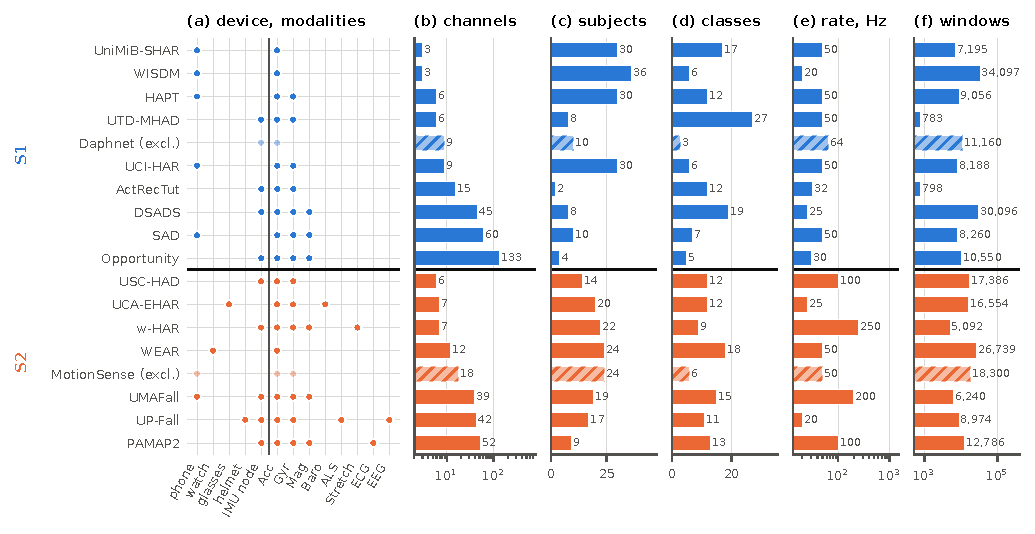
\includegraphics[width=\textwidth]{figures/fig04_sensors.pdf}
\caption{Sensor configuration of the datasets of S1 (development) and S2 (held-out). (a) Devices and sensor
modalities, quoted from the benchmark's dataset table~\cite{burzer2026arena}; (b)--(f) channels, subjects, classes,
sampling rate and number of 3-s windows (logarithmic axes in (b), (e) and (f)), read from the stored runs and the
harness's splits. Faded and hatched: excluded from the variance analyses by the pre-registered inclusion rule.}
\label{fig:sensors}
\end{figure*}

\begin{table*}[t]
\caption{Datasets of the stored runs}
\label{tab:datasets}
\centering
\footnotesize
\begin{tabular}{@{}llllrrrrrr@{}}
\toprule
Dataset & Set & Device & Modalities & $C$ & Subj. & Cl. & Hz & Windows & Splits \\
\midrule
UniMiB-SHAR & S1 & phone & Acc & 3 & 30 & 17 & 50 & 7,195 & 10 \\
WISDM & S1 & phone & Acc & 3 & 36 & 6 & 20 & 34,097 & 10 \\
HAPT & S1 & phone & Acc, Gyr & 6 & 30 & 12 & 50 & 9,056 & 10 \\
UTD-MHAD & S1 & node & Acc, Gyr & 6 & 8 & 27 & 50 & 783 & 8 \\
Daphnet$^\dagger$ & S1 & node & Acc & 9 & 10 & 3 & 64 & 11,160 & 10 \\
UCI-HAR & S1 & phone & Acc, Gyr & 9 & 30 & 6 & 50 & 8,188 & 10 \\
ActRecTut & S1 & node & Acc, Gyr & 15 & 2 & 12 & 32 & 798 & 2 \\
DSADS & S1 & node & Acc, Gyr, Mag & 45 & 8 & 19 & 25 & 30,096 & 8 \\
SAD & S1 & phone & Acc, Gyr, Mag & 60 & 10 & 7 & 50 & 8,260 & 10 \\
Opportunity & S1 & node & Acc, Gyr, Mag & 133 & 4 & 5 & 30 & 10,550 & 4 \\
\midrule
USC-HAD & S2 & node & Acc, Gyr & 6 & 14 & 12 & 100 & 17,386 & 10 \\
UCA-EHAR & S2 & glasses & Acc, Gyr, Baro & 7 & 20 & 12 & 25 & 16,554 & 10 \\
w-HAR & S2 & node & Acc, Gyr, Mag, Stretch & 7 & 22 & 9 & 250 & 5,092 & 10 \\
WEAR & S2 & watch & Acc & 12 & 24 & 18 & 50 & 26,739 & 10 \\
MotionSense$^\dagger$ & S2 & phone & Acc, Gyr & 18 & 24 & 6 & 50 & 18,300 & 10 \\
UMAFall & S2 & node, phone & Acc, Gyr, Mag & 39 & 19 & 15 & 200 & 6,240 & 10 \\
UP-Fall & S2 & node, helmet & Acc, Gyr, ALS, EEG & 42 & 17 & 11 & 20 & 8,974 & 10 \\
PAMAP2 & S2 & node & Acc, Gyr, Mag, ECG & 52 & 9 & 13 & 100 & 12,786 & 9 \\
\bottomrule
\end{tabular}
\\[2pt]
\parbox{\textwidth}{\footnotesize $C$: channels; Subj.: subjects; Cl.: classes; Hz: sampling rate; Windows: 3-s windows,
each in one test group; Splits: test-subject groups. $^\dagger$Excluded from the variance analyses by the
pre-registered inclusion rule.}
\end{table*}

\subsection{Protocol and stored runs}
All runs follow WHAR Arena v1 with its paper-era code~\cite{burzer2026arena,burzer2025whar}: 3-s windows with 50\,\%
overlap at the native sampling rate; $k=10$ subject groups, each split testing on one group
(1 to 4 subjects) that never appears in training or validation;
validation from 20\,\% of the training subjects' windows, drawn window by window, so that a validation window can
share half its samples with a training window; a z-score fitted on the training split; macro-F1 over all
classes, with classes absent from a test split counted as 0. Apart from a label-permutation control, no network was
trained for this letter: we analyse stored runs and their checkpoints. Three sets enter (Table~\ref{tab:vc}): S1, ten networks that share one skeleton and differ
in single components (with and without temporal memory, e.g.\ S4D~\cite{gu2022efficiently,gu2022parameterization} and
Mamba~\cite{gu2023mamba}, or window statistics), on ten development datasets with three seeds; S2, four of these
networks on eight datasets not used to find the effect, with three seeds (Section~\ref{sec:choice}); S3, the
benchmark's 17 published models
(deep networks such as DeepConvLSTM~\cite{ordonez2016deep,hammerla2016deep}, and Random Forest~\cite{breiman2001random},
SVM and k-NN on tsfresh features~\cite{christ2018tsfresh}) re-run with the same code on four datasets, one run per
split. A pre-registered inclusion rule removed datasets whose stored runs disagree on split sizes, because their split
indices do not name the same subjects across runs (one dataset each in S1 and S2). Fig.~\ref{fig:design} summarises
the design, the runs analysed and how subjects are assigned to test groups.

\begin{figure*}[t]
\centering
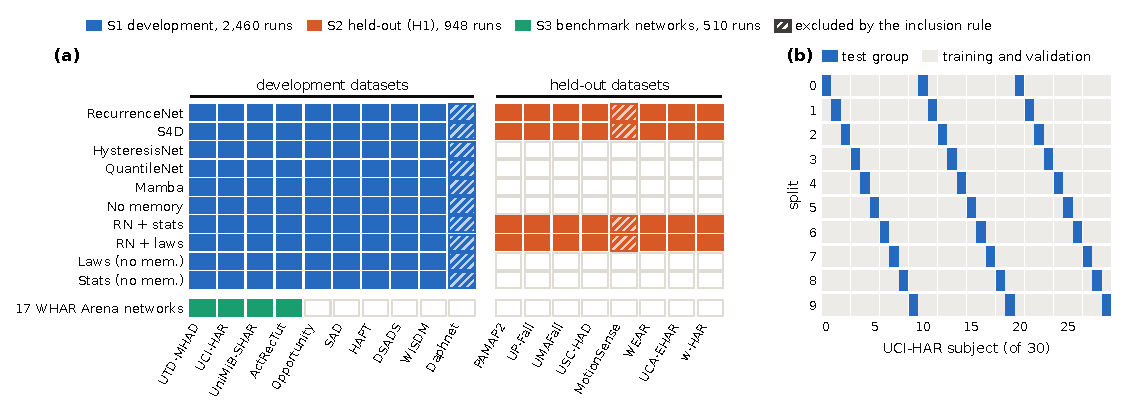
\includegraphics[width=\textwidth]{figures/fig03_design.pdf}
\caption{Study design. (a) From the stored runs to the variance decomposition. (b) The runs: networks (rows) by
datasets (columns), coloured by run set; each cell gives splits $\times$ seeds, and hatched cells are excluded by the
inclusion rule. (c) The person-disjoint test groups of UCI-HAR: each split tests on three subjects that never enter its
training or validation data.}
\label{fig:design}
\end{figure*}

\subsection{Networks}
The ten networks of S1 and S2 share one skeleton (Fig.~\ref{fig:arch}, Table~\ref{tab:models}). A linear encoder maps
the $C$ channels of each sample to $D$ features, $N$ residual blocks process the sequence, and the features are
averaged over the window, joined in four networks by a window-level side path, normalised (LayerNorm) and classified by
a linear head. The vector the head receives is the network's embedding (Section~\ref{sec:emb}). In a residual block, a
LayerNorm and a linear map give per-channel signals $u$ that feed a memory; $u$ and the memory's outputs are
concatenated, mixed linearly and passed through a GELU into the residual sum. RecurrenceNet's memory keeps soft rows of
a recurrence plot~\cite{eckmann1987recurrence} over ten lags: whether a learned two-dimensional projection of the
signal is back where it was $\tau$ samples earlier. HysteresisNet keeps four play operators per channel, whose output
moves only when the input leaves a band of half-width $r$ around it~\cite{brokate1996hysteresis} (here with
input-dependent widths and a clock channel). QuantileNet keeps four online quantile trackers per channel, stochastic
approximation steps~\cite{robbins1951stochastic} that settle on a running quantile of level $\tau$. The no-memory
control sets every play width to zero, which makes each operator the identity, and the two networks without memory
use plain blocks. S4D~\cite{gu2022parameterization} and Mamba~\cite{gu2023mamba} use their own blocks, a diagonal
state-space convolution and a selective scan. The side paths read per-channel window statistics (mean, standard
deviation, minimum and maximum, the kind of features behind the Random Forest) or invariants of each three-axis
sensor's temporal operator and of the couplings between sensors (``laws''). With the reference input of gate G1 (that
of UTD-MHAD), the networks have 17,931 to 27,675 parameters, and on the
datasets of S1 and S2 15,678 to 49,437. RN + laws is the RILA-Net of the
companion study~\cite{le2026rila}, which describes these networks in full and compares them.

\begin{figure*}[t]
\centering
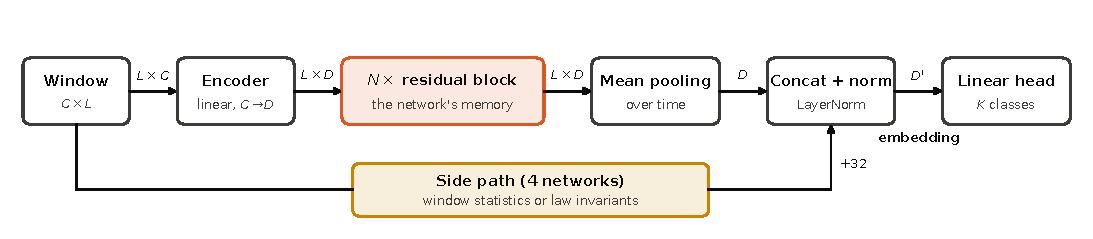
\includegraphics[width=\textwidth]{figures/fig05_architecture.pdf}
\caption{The networks of S1 and S2 as a dataflow diagram. (a) The shared skeleton, with the tensor shapes on its
edges ($C$ channels, $L$ samples, width $D$, $K$ classes); the embedding analysed in Section~\ref{sec:emb} is the
head's input. (b) The residual block with its skip connection; the memory returns $F$ features per channel. (c) Each
memory's update per channel and time step, the state it keeps, and the networks that use it (sizes in
Table~\ref{tab:models}).}
\label{fig:arch}
\end{figure*}

\begin{table}[t]
\caption{The ten networks}
\label{tab:models}
\centering
\setlength{\tabcolsep}{2pt}
\resizebox{\columnwidth}{!}{\begin{tabular}{@{}llllrrrr@{}}
\toprule
Network & Memory & Side path & Sets & $D{\times}N$ & Emb. & Params (ref.) & Range over datasets \\
\midrule
RecurrenceNet & recurrence & none & S1, S2 & 32$\times$3 & 32 & 24,675 & 23,886--28,013 \\
S4D & S4D (diagonal SSM) & none & S1, S2 & 64$\times$2 & 64 & 27,675 & 26,118--34,373 \\
HysteresisNet & play operators & none & S1 & 32$\times$3 & 32 & 23,579 & 22,790--26,917 \\
QuantileNet & quantile trackers & none & S1 & 32$\times$3 & 32 & 20,763 & 19,974--24,101 \\
Mamba & Mamba (S6) & none & S1 & 32$\times$2 & 32 & 21,147 & 20,358--24,485 \\
No memory & none (play width 0) & none & S1 & 32$\times$3 & 32 & 19,995 & 19,206--23,333 \\
RN + stats & recurrence & channel stats & S1, S2 & 32$\times$3 & 64 & 26,451 & 24,582--46,357 \\
RN + laws & recurrence & law invariants & S1, S2 & 32$\times$3 & 64 & 27,553 & 25,316--49,437 \\
Laws (no mem.) & none (plain block) & law invariants & S1 & 48$\times$3 & 80 & 19,033 & 16,412--42,597 \\
Stats (no mem.) & none (plain block) & channel stats & S1 & 48$\times$3 & 80 & 17,931 & 15,678--39,517 \\
\bottomrule
\end{tabular}
}\\[2pt]
\parbox{\columnwidth}{\footnotesize Emb.: embedding dimension. Params (ref.): with the reference input of gate G1;
range over the datasets of S1 and S2.}
\end{table}

\subsection{Why these networks}\label{sec:choice}
A confirmatory estimate of $R$ needs runs with four properties, and the choice of networks follows from them.
(i) Several training seeds on every split: without them the network $\times$ split interaction cannot be told from
seed noise, and the subject-to-network ratio can only be bounded conservatively, as on S3. (ii) Per-split results
paired across networks on datasets that did not suggest the hypothesis: the decomposition rests on every network
seeing the same test subjects, and a confirmatory test must not reuse the data it came from. (iii) Networks that
differ in controlled, single components at similar size, so that the network terms measure the differences between
competitive design choices, the decision a sensing study usually faces, rather than differences of capacity, input
pipeline or model family. (iv) No new training, fixed in the pre-registration, so that the confirmatory data could
not be shaped after the hypothesis was stated.

The benchmark's networks do not meet (i) and (ii). The benchmark trains one run per split, its published results give
only means and standard deviations over splits~\cite{burzer2026arena}, and per-split results of its 17 networks are
available to us only on four development datasets of S1 (set S3). Training them anew on held-out datasets with
several seeds would have broken (iv). Among the stored runs, only S2 meets all four properties: three seeds on every
split of eight datasets outside the development set, for four networks of one skeleton with 24,675
to 27,675 parameters on the reference input. They form two single-component contrasts and
one change of memory family: RecurrenceNet; the same network with a side path of window statistics (RN + stats) or of
law invariants (RN + laws); and S4D, a published diagonal state-space memory~\cite{gu2022parameterization}. Three of
the four thus share RecurrenceNet's memory, and the network terms of S2 measure side paths and one alternative memory,
not the full range of published architectures. We produced these runs before this study, as the pre-registered
held-out evaluation of the companion study~\cite{le2026rila}, which reports these networks' accuracies and paired
differences; they were therefore known when H1 was registered, whereas the variance components were not. This letter
reuses the runs for a different question and reports no comparison between the networks. The benchmark's networks enter as S3, an independent population with which we test how far the
result extends (Section~\ref{sec:pop}).

How comparable the four are, and where they stand, was measured afterwards (r). On the 7
datasets of H1 their means span 58.0 to 63.2 F1 points, and within a
dataset they differ by a median of 7.2 points (at most 9.9, on
UMAFall), against 27.0 for the benchmark's 17
published networks on the same datasets. Placed among those, whose means span 42.2 to
64.9, the four would rank between 5th and 13th:
neither the benchmark's strongest nor its weakest networks. This comparison sets three-seed means against published
single runs of the same protocol; it locates the population and ranks no network.

\subsection{Variance model and pre-registered test}
For run $(m,d,s,r)$ of network $m$ on split $s$ of dataset $d$ with seed $r$,
\begin{equation}
y_{mdsr} = \mu_d + P_{ds} + M_m + (MD)_{md} + (MP)_{mds} + e_{mdsr},\label{eq:model}
\end{equation}
with $\mu_d$ fixed and the other terms independent zero-mean random effects, fitted by REML~\cite{patterson1971recovery}
in statsmodels~\cite{seabold2010statsmodels}. The estimand is $R=\sigma^2_P/(\sigma^2_M+\sigma^2_{MD}+\sigma^2_{MP})$,
the variance of the test-subject group over all network-related variance; $\pi_P$ is $\sigma^2_P$'s share of the
within-dataset variance. A split changes the test subjects and, with them, the training and validation subjects, so
$P$ is the effect of the subject partition. On the datasets of S2, with nine or ten groups, any two splits share most
of their training subjects, so $P$ is mainly the effect of the test group. Intervals are percentile 97.5\,\% intervals from 1000 cluster-bootstrap
resamples that draw splits within datasets~\cite{field2007bootstrapping}; they treat the networks as fixed. Before any
variance analysis of S2, we registered H1 ($R>1$ on S2), with success if the interval's lower bound exceeds 1 and
failure if $R\le 1$, sealed the analysis code by hash, and logged S2's single read. S2's per-dataset means and its
paired network differences were known (Section~\ref{sec:choice}); its variance components were not. For S3 (one run per
split) the interaction and the seed cannot be separated, so the conservative
$R'=\sigma^2_P/(\sigma^2_M+\sigma^2_{MD}+\sigma^2_e)$ is reported.

\subsection{Exploratory analyses}
None of the following analyses was pre-registered. Those marked (r), here and in Section~\ref{sec:choice}, were
added after an internal review.

\emph{Network population (r).} We refit S3's model to sub-populations of its networks: the 14 deep networks, and the
$k$ best networks for $k$ from 3 to 17, ranked by their mean published macro-F1 on the 26 Arena
datasets outside S3~\cite{burzer2026arena}, so that the ranking reads no score of the runs analysed. Each point
estimate keeps the better of the statsmodels fit and an independent REML implementation; intervals use the bootstrap
of H1.

\emph{Error budget (r).} Under \eqref{eq:model}, the difference between two networks on one dataset, averaged over $k$ test-subject
groups and $n$ seeds, has a true part with variance $2(\sigma^2_M+\sigma^2_{MD})$ over pairs of networks and a noise
part with variance $2(\sigma^2_{MP}+\sigma^2_e/n)/k$ when both networks run on the same splits (paired), and
$2(\sigma^2_P+\sigma^2_{MP}+\sigma^2_e/n)/k$ when they run on different test subjects (unpaired, e.g.\ two studies
that each report one hold-out split). From the point estimates we derive the noise SD, the smallest true difference a
two-sided test at 5\,\% detects with 80\,\% power, and the reliability (true over
true plus noise variance). $k$ beyond 10 means more groups of the same size, that is, more recorded subjects.

\emph{Validation against the test (r).} For each dataset of S1 and S2 whose runs all recorded a validation score, we
rank-correlate the networks' validation and test means, and compare this with how well the test ranking agrees with
itself: test means of seed 0 against seeds 1--2 (same splits), and of the even against the odd splits (other test
subjects).

\emph{Further analyses.} Over the
benchmark's 30 datasets we regress the published single-run results on standardised dataset properties (ordinary least
squares; four properties, four outcomes); these associations are correlational, and we report Holm-adjusted
$p$-values over the 16 coefficient tests~\cite{holm1979simple} (r). Within each dataset of S1 and S2 we
compare the spread of the split means (over networks and seeds) with that of the network means (over splits and
seeds).

\subsection{Embedding analysis}\label{sec:emb}
This analysis is exploratory and uses inference only. For the seed-0 checkpoint of every split of the
11 datasets whose caches on our cluster reproduce the stored runs (eight of S1 with the ten networks,
three of S2 with four), the harness rebuilds the split and the network embeds every training and test window; the
regenerated macro-F1 equals the stored one in 686 of 754 cases (largest
difference 0.20 points). Three quantities describe each network and
split. First, the class-conditional shift of the test group~\cite{zhang2013domain}: for every class present in both,
the distance between the test and the training class means, in units of the training class's root-mean-square spread
per dimension, averaged over classes. The same shift is computed in a sensor-feature space that no network shapes
(per-channel mean, standard deviation, minimum and maximum of the normalised window). Second, the subject information
in the training embeddings: the balanced accuracy of a linear probe~\cite{alain2016understanding} (logistic
regression) that predicts the training subject, in five folds grouped by recording session so that overlapping
windows never straddle folds, on at most 4,000 windows, against chance (one over the number of
training subjects). Third, the same probe for the activity. Within each dataset we rank-correlate the test group's
shift, averaged over networks, with the split's macro-F1 (Spearman), and we pool the within-dataset ranks over
datasets with more than three splits. One case, fixed before the analysis (UCI-HAR, S4D, split~0), is mapped to two
dimensions with t-SNE~\cite{vandermaaten2008visualizing}.

\subsection{Verification}
For verification, the
benchmark's Random Forest, re-run with our code, reproduces its published macro-F1 on four datasets (e.g.\
84.69 against 84.69 on UCI-HAR); test predictions were regenerated from
408 checkpoints, 373 of which reproduced the stored metrics exactly and all within two
test windows; an independent REML implementation and negative controls (e.g.\ permuting network labels within cells)
confirmed the analysis; and S4D retrained on permuted training labels (6 runs on UP-Fall and UCA-EHAR)
fell to chance, with a test macro-F1 of 4.9 against 8.7
by chance and 54.5 with the true labels. Of the 828 confirmatory runs, the gate
regenerated 360 on the caches the stored runs used, within that tolerance. Beyond the gate, every analysed run
with a checkpoint was re-executed (2,982 of 2,988):
2,185 reproduce their records exactly, 2,668 within two test
windows, and none differs by more than 3.25 F1 points. The residual
differences have one source. Several parsers number activities and subjects, and order recordings, in the order the
file system lists them, and many stored runs were built on cloud machines whose listing order cannot be recreated.
For DSADS we recovered that order from the checkpoints themselves, since each network is near-perfect on its own
training subjects, which identifies its output labels and its test subjects, and rebuilt the cache accordingly; for
USC-HAD and three datasets whose caches we rebuilt, the test sets are identical and only the draw of validation
windows, and with it the train-only z-score, differs. The 6 runs without a checkpoint were retrained to obtain one;
5 of them reproduce their record's macro-F1 exactly, and the stored records remain the
ones analysed. The companion study~\cite{le2026rila} instead retrained the runs it could not re-execute, without
recovering their listing order; the two papers therefore analyse different values for three runs of H1 (two of w-HAR, one of
USC-HAD), for the seed-2 runs of three networks on DSADS, and for runs of MotionSense and Daphnet, which our inclusion
rule excludes.

\section{Results}
\subsection{Confirmatory test}
On S2 the test-subject group dominates (Fig.~\ref{fig:vc}, Table~\ref{tab:vc}): $\sigma^2_P=127.7$
(F1 points$^2$) against $\sigma^2_M=4.8$, $\sigma^2_{MD}=4.0$ and $\sigma^2_{MP}=6.9$,
with the seed at $\sigma^2_e=11.7$. Hence $R=8.19$ [2.85, 16.90] and
$\pi_P=82$\,\% [64, 89]: the pre-registered decision is \emph{success},
and the secondary criterion ($\pi_P$ lower bound $\ge 40$\,\%) is met.

\begin{figure}[t]
\centering
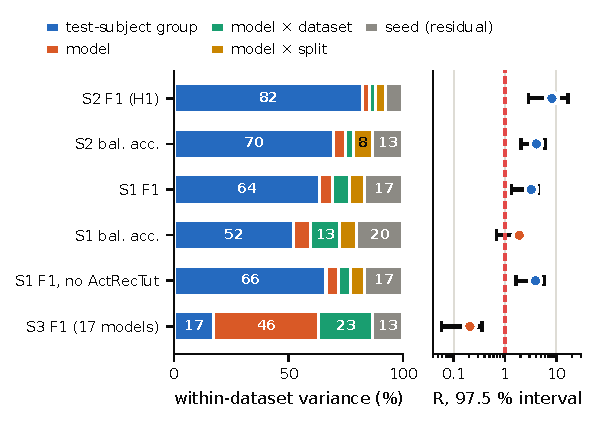
\includegraphics[width=\columnwidth]{figures/fig01_variance_components.pdf}
\caption{Where the within-dataset variance of the stored runs lies. Left: shares by source (numbers in \%; the seed
term, grey, is the residual). Right: $R$ with its 97.5\,\% bootstrap interval, blue where the interval lies above 1
and orange otherwise; the dashed line is the pre-registered threshold. $R$ exceeds 1 in every
analysis of the shared-skeleton networks (on S1 with balanced accuracy its interval includes 1), and the network
dominates across the 17 heterogeneous published architectures (S3, conservative $R'$; by population in
Fig.~\ref{fig:pop}a).}
\label{fig:vc}
\end{figure}

\begin{table}[t]
\caption{Variance components (F1 points$^2$) and $R$ [97.5\,\% interval]}
\label{tab:vc}
\centering
\setlength{\tabcolsep}{3pt}
\resizebox{\columnwidth}{!}{\begin{tabular}{@{}lrrrrrrl@{}}
\toprule
Analysis & $n$ & $\sigma^2_P$ & $\sigma^2_M$ & $\sigma^2_{MD}$ & $\sigma^2_{MP}$ & $\sigma^2_e$ & $R$ [97.5\,\% int.] \\
\midrule
S2 F1 (H1) & 828 & 127.7 & 4.8 & 4.0 & 6.9 & 11.7 & 8.19 [2.85, 16.90] \\
S2 bal. acc. & 828 & 86.3 & 6.5 & 4.4 & 10.1 & 16.6 & 4.09 [2.05, 6.03] \\
S1 F1 & 2160 & 66.2 & 5.9 & 7.8 & 6.7 & 17.6 & 3.26 [1.34, 4.47] \\
S1 bal. acc. & 2160 & 39.2 & 5.5 & 9.6 & 5.5 & 15.3 & 1.89 [0.69, 2.29] \\
S1 F1, no ActRecTut & 2100 & 67.4 & 5.5 & 5.1 & 6.5 & 17.0 & 3.93 [1.63, 5.80] \\
S3 F1 (17 models) & 510 & 37.5 & 100.2 & 51.0 & -- & 29.2 & 0.21 [0.06, 0.36] \\
\bottomrule
\end{tabular}
}
\end{table}

\subsection{Sensitivity analyses}
Balanced accuracy, which averages recall over the classes present and so has no per-split ceiling, gives
$R=4.09$ [2.05, 6.03]
on S2: ceilings enlarge the subject share but do not create it. On the development set S1 the ordering is the same
with macro-F1 ($R=3.26$ [1.34, 4.47]), also
without its two-subject dataset ActRecTut ($R=3.93$); with balanced accuracy the point
estimate stays above 1 but the interval does not exclude it ($R=1.89$
[0.69, 2.29]). Across the benchmark's 17 published architectures
it reverses: $R'=0.21$ [0.06, 0.36], with
$\sigma^2_M=100.2$ against $\sigma^2_P=37.5$. These architectures range
from k-NN to attention networks; Section~\ref{sec:pop} shows which of them cause the reversal.

\subsection{Which networks are compared}\label{sec:pop}
This analysis is exploratory (r). The reversal on S3 comes from the networks at the bottom of the benchmark
(Fig.~\ref{fig:pop}a). Ranked by their published macro-F1 on other datasets, the best $k$ networks keep $R'$ above 1
up to $k=12$: for the best five $R'=1.86$ [0.36,
3.94], for the best 12 $R'=1.26$ [0.32,
2.25], although no interval excludes 1 (0 of 15
populations). Adding the three weakest deep networks of the ranking (DeepConvShallowLSTM, Guan-LSTM, SA-HAR) lowers it
to $0.36$, and SVM and k-NN to $0.21$; from the 13th network on, every
interval lies below 1 (5 populations). The classical baselines alone do not explain the
reversal: the 14 deep networks give $R'=0.34$ [0.10,
0.64], and their largest term is the network $\times$ dataset interaction
($\sigma^2_{MD}=56.4$, against $\sigma^2_M=37.5$ and $\sigma^2_P=42.7$;
Fig.~\ref{fig:pop}b). Across the published deep networks, which network suits which dataset outweighs both who is
tested and which network is best overall.

\begin{figure*}[t]
\centering
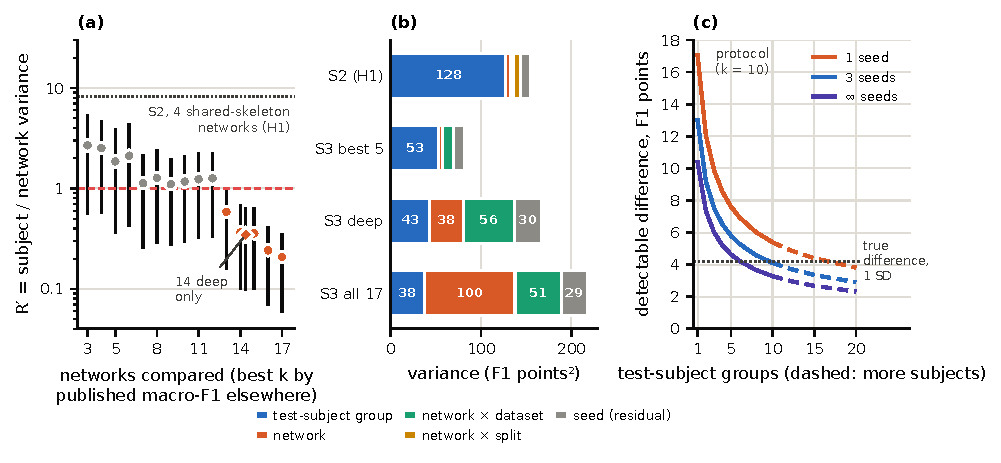
\includegraphics[width=\textwidth]{figures/fig10_population_budget.pdf}
\caption{Exploratory, added after review. (a) $R'$ of S3 with its 97.5\,\% bootstrap interval for the $k$ best of the
benchmark's 17 networks, ranked by their mean published macro-F1 on the 26 Arena datasets
outside S3 (circles), and for its 14 deep networks (diamond); blue where the interval lies above
1, orange below 1, grey across 1. Dotted: $R$ of the pre-registered test (S2). (b) Variance components of S2 and of
three S3 populations: the test-subject group dominates among comparable networks, the network $\times$ dataset
interaction among the deep ones. (c) The smallest network difference a paired comparison detects (two-sided
5\,\% test, 80\,\% power) by number of test-subject groups and seeds, from S2's
components; dashed beyond the protocol's ten groups (more subjects); dotted, the SD of the true difference between two
networks. An unpaired single-split comparison would need 47.9 points.}
\label{fig:pop}
\end{figure*}

\subsection{Error budget of a comparison}
This analysis is exploratory (r). With S2's components (Table~\ref{tab:budget}, Fig.~\ref{fig:pop}c), the true
difference between two of its networks on a dataset has an SD of 4.2 F1 points. A comparison on one
split and one seed has a noise SD of 6.1 points when both networks see the same test
subjects, and of 17.1 when they do not, as when two studies each report one hold-out
split: reliabilities of 0.32 and 0.06. The protocol's ten
groups and three seeds, paired, bring the noise SD to 1.5 points (detectable difference
4.1, reliability 0.89): a typical difference
between comparable networks lies at the limit of what one dataset can show. More seeds would remove at most
20\,\% of this noise, because the network $\times$ split interaction sets a floor of
1.2 points; twice as many test-subject groups would remove 29\,\%.
A single network's dataset mean estimates its accuracy on new people of the same population with a standard error of
3.7 points, close to the typical difference between two networks. The development set S1 gives the
same picture (Table~\ref{tab:budget}).

\begin{table}[t]
\caption{Error budget of a comparison between two networks (F1 points)}
\label{tab:budget}
\centering
\setlength{\tabcolsep}{3pt}
\resizebox{\columnwidth}{!}{\begin{tabular}{@{}lrrrrrr@{}}
\toprule
 & \multicolumn{3}{c}{S2 (held-out)} & \multicolumn{3}{c}{S1 (development)} \\
\cmidrule(lr){2-4}\cmidrule(l){5-7}
Comparison & SD & Detect. & Rel. & SD & Detect. & Rel. \\
\midrule
Unpaired, 1 $\times$ 1 & 17.1 & 47.9 & 0.06 & 13.5 & 37.7 & 0.13 \\
Paired, 1 $\times$ 1 & 6.1 & 17.1 & 0.32 & 7.0 & 19.5 & 0.36 \\
Paired, 10 $\times$ 1 & 1.9 & 5.4 & 0.82 & 2.2 & 6.2 & 0.85 \\
Paired, 10 $\times$ 3 (protocol) & 1.5 & 4.1 & 0.89 & 1.6 & 4.4 & 0.92 \\
Paired, 10 $\times$ $\infty$ & 1.2 & 3.3 & 0.93 & 1.2 & 3.2 & 0.95 \\
Paired, 20 $\times$ 3 & 1.0 & 2.9 & 0.94 & 1.1 & 3.1 & 0.96 \\
\midrule
True difference of two networks, SD & \multicolumn{3}{l}{4.2} & \multicolumn{3}{l}{5.2} \\
\bottomrule
\end{tabular}
}\\[2pt]
\parbox{\columnwidth}{\footnotesize Exploratory, from the point estimates of Table~\ref{tab:vc}. Comparison: test-subject
groups $\times$ seeds; paired: both networks on the same splits. SD: noise SD of the difference; Detect.: smallest true
difference detected by a two-sided 5\,\% test with 80\,\% power; Rel.: reliability,
true over true plus noise variance. Twenty groups means more recorded subjects.}
\end{table}

\subsection{Spread across test groups and networks}
The decomposition's result is visible in the raw means (Fig.~\ref{fig:spread}a). In 15
of 16 datasets of S1 and S2 the split means vary more than the network means, by a median factor of
2.6 in standard deviation; the exception is ActRecTut, whose two splits each test one of its two
subjects. On UCI-HAR the split means have a standard deviation of 3.0 F1 points against
1.5 for the network means, and on UP-Fall 8.3 against
4.4. In the network $\times$ split cells (Fig.~\ref{fig:spread}b, c) the columns
dominate: a test group that is hard for one network is hard for the others.

\begin{figure*}[t]
\centering
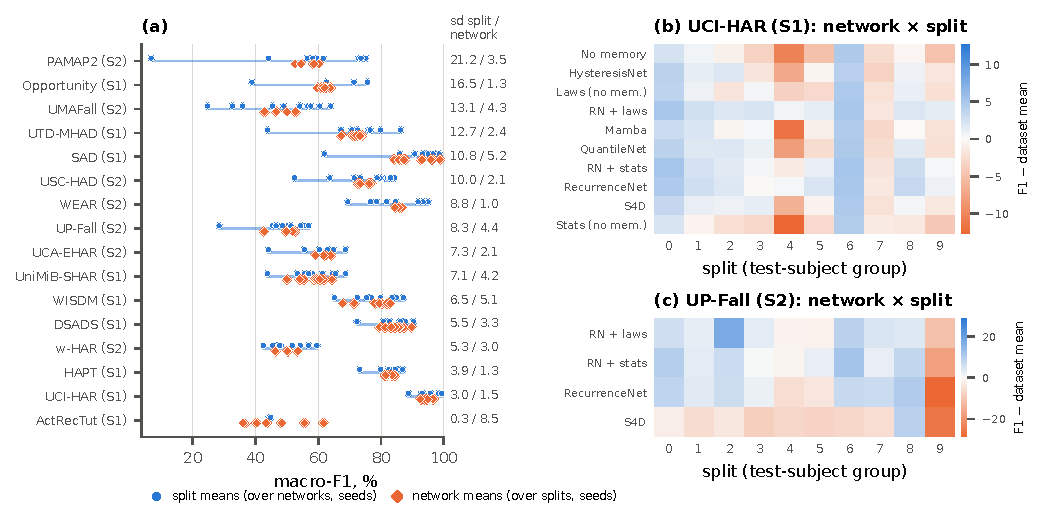
\includegraphics[width=\textwidth]{figures/fig07_split_spread.pdf}
\caption{Exploratory. (a) Within each dataset of S1 and S2, the means of the splits (circles; over networks and
seeds) and of the networks (diamonds; over splits and seeds); right, the standard deviation of each. (b, c) Network
$\times$ split cell means (over seeds) of UCI-HAR and UP-Fall, as deviations from the dataset mean.}
\label{fig:spread}
\end{figure*}

\subsection{Validation on the training subjects}\label{sec:val}
Each run's validation windows are drawn, window by window, from its training subjects' recordings: they come from
people the network has seen and can overlap its training windows, so the gap below mixes both
effects~\cite{hammerla2015lets} (Fig.~\ref{fig:val}). On the 13 datasets whose runs all recorded it,
the validation macro-F1 exceeds the test macro-F1 in 2,307 of 2,388 runs, by a median
of 17.1 points per dataset (from 4.6 to 47.8); the four largest gaps are on
held-out datasets. The validation score is also a poor guide to the networks' test ranking, whereas the test ranking
agrees with itself (r). The rank correlation between the networks' validation and test means has a median of
$+0.18$ over the 13 datasets, against $+0.80$
between the test means of different seeds and $+0.80$ between those of different test
subjects (even against odd splits); it is below the split-half value in 9
datasets. The network best on validation is the best on test in 3 of
13 datasets, the network best on the even splits the best on the odd ones in
7. On the odd splits, choosing by validation loses a median of
3.3 points, choosing by the even splits
0.0.

\begin{figure*}[t]
\centering
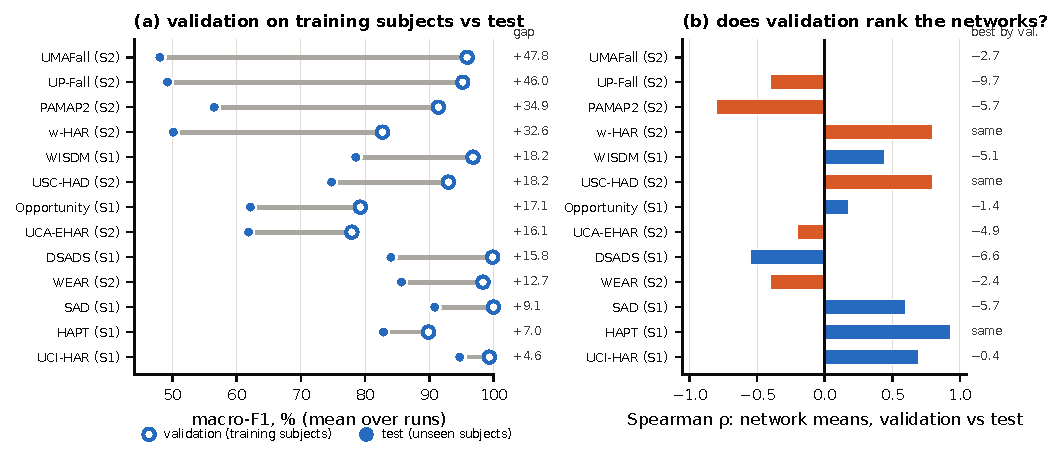
\includegraphics[width=\textwidth]{figures/fig09_validation.pdf}
\caption{Exploratory. (a) Per dataset, the mean validation macro-F1 (windows of the training subjects) and the mean
test macro-F1 (unseen subjects) of the stored runs, and their gap. (b) Spearman correlation between the networks'
validation and test means (S1 blue, S2 orange); right, whether the network best on validation is also best on test,
or how many test points the choice loses. Datasets whose runs did not all record a validation score are omitted.}
\label{fig:val}
\end{figure*}

\begin{figure}[t]
\centering
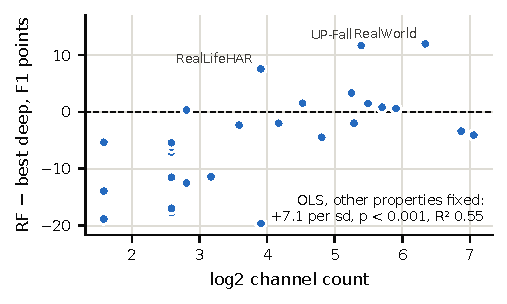
\includegraphics[width=\columnwidth]{figures/fig02_channels.pdf}
\caption{Exploratory. Over the benchmark's 30 datasets (published single runs), the Random Forest's margin over the
best deep network rises with the number of sensor channels.}
\label{fig:explore}
\end{figure}

\subsection{Exploratory findings}
Which components of these networks matter (a temporal memory, its type, the side paths), and what their memories
learn, is the subject of the companion study~\cite{le2026rila}; this letter reports no architecture contrast.

Over the 30 datasets, a larger channel count goes with a larger margin of the feature-based Random Forest over the
best deep network ($+7.1$ points per standard deviation of $\log_2$ channels, other properties
held fixed, Holm-adjusted $p< 0.001$; Fig.~\ref{fig:explore}). Of the 16 tests,
2 survive the correction: this one and the association of channel count with the spread
over test-subject groups (adjusted $p= 0.025$). Fewer subjects go with a larger gap between the
best and the median deep network ($-1.5$ per standard deviation, uncorrected
$p= 0.004$), but not after the correction (adjusted $p= 0.058$); this gap, a
maximum over noisy means, also rises with the spread over test groups ($\rho=+0.60$,
$p< 0.001$), so it may reflect noisier estimates rather than larger network differences (r). No property
predicts how hard a dataset is ($R^2=0.03$).

\subsection{Embeddings}
The hard test groups are the distant ones (Fig.~\ref{fig:emb}). In a sensor-feature space that no network shapes
(window statistics of the normalised signal), the splits whose test subjects lie further from the training subjects,
class by class, are the splits on which the networks score lower: the pooled within-dataset rank correlation is
$\rho=-0.32$ ($p= 0.002$),
negative in 9 datasets. In the networks' embeddings the association is stronger,
as it must partly be in the space the classifier reads: $\rho=-0.46$
($p< 0.001$), negative in 10 of
10 datasets (median $-0.61$) and, for single
networks, in 69 of 82 network--dataset pairs (median
$-0.50$); per embedding dimension, so that networks of different width weigh
alike, $\rho=-0.45$. The training embeddings still carry
the subject's identity, as known for deep HAR features~\cite{iwasawa2017privacy}: a linear probe identifies the
training subject at a median 3.2 times chance, against
4.0 times from the window statistics, while the activity probe reaches a
median balanced accuracy of 99\,\%. The networks thus reduce the subject
information in their features without removing it. These associations are exploratory and correlational.

\begin{figure*}[t]
\centering
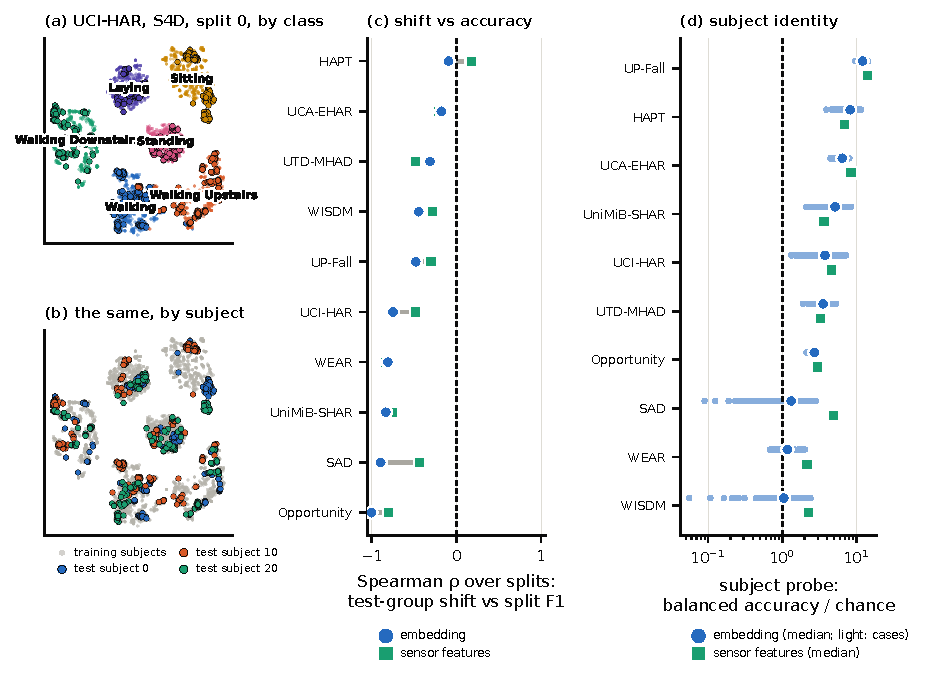
\includegraphics[width=\textwidth]{figures/fig08_embedding.pdf}
\caption{Exploratory embedding analysis (seed-0 checkpoints, inference only). (a, b) t-SNE of the embeddings of one
case fixed in advance (UCI-HAR, S4D, split~0): training windows (small, faded; a seeded subsample) and the test
windows of the three unseen subjects (outlined), coloured by activity (a) and by subject (b). (c) Per dataset, Spearman
correlation over splits between the test group's class-conditional shift (mean over networks) and the split's
macro-F1, in the embedding and in a sensor-feature space. (d) Balanced accuracy of a linear probe that identifies the
training subject, over chance, from the embeddings (all cases and median) and from the window statistics (median).}
\label{fig:emb}
\end{figure*}

\clearpage  % working draft: place every pending figure before the discussion and the references
\raggedbottom  % working draft: do not stretch the short column after the float page
\section{Discussion and Limitations}
\emph{What is new.} That accuracy varies widely between people was known~\cite{barshan2016investigating,jordao2018human};
how that variation compares with the differences between networks, and what it implies for a comparison, was not.
The decomposition answers both under one protocol. For networks that differ in single components, so that their
means differ by a median of 7.2 points within a dataset, who is tested decides more of
a reported macro-F1 than which network is used, as the pre-registered test confirmed on held-out data. These networks
sit in the middle and upper part of the benchmark (ranks 5 to 13 of
17 on the same datasets), roughly the region where S3's ratio stays near or above 1. The ratio is not a
constant of wearable HAR but a property of the networks compared: it holds near or above 1 among the benchmark's
best published networks and reverses once weaker ones enter, and among the published deep networks the largest term is the network $\times$ dataset
interaction, a quantitative form of the benchmark's finding that no architecture leads everywhere~\cite{burzer2026arena}.

\emph{What it implies for a study.} The variance between test-subject groups governs the absolute level, and with it
every comparison made across studies, splits or subject groups: an unpaired comparison on one hold-out split has a
reliability of 0.06 (Table~\ref{tab:budget}). A comparison paired by split cancels it,
but is then limited by the network $\times$ split interaction and the seed, which on S2 are as large as the network
terms themselves (Table~\ref{tab:vc}). Hence four rules for a wearable sensing study. Compare networks paired on the
same splits, never by means over different subjects. Size the comparison by test subjects: with the protocol's ten
groups and three seeds, about 4.1 F1 points are detectable on one dataset,
and further seeds cannot go below the floor that the network $\times$ split interaction sets. Select networks and stop
training on held-out subjects, since validation windows of the training subjects rank networks far worse than the test
ranks them against itself (Section~\ref{sec:val}). Report the spread across test-subject groups, and the standard
error of a mean as an estimate for new people (3.7 points on S2), with every score.

\emph{Exploratory evidence.} Within datasets, test groups spread accuracy more than networks do
(Fig.~\ref{fig:spread}). A test group is hard when its windows, class by class, lie far from the training subjects',
already in features that no network shapes, and the networks' embeddings still identify the training subjects
(Fig.~\ref{fig:emb}). Together these suggest that, for comparable networks, the training subjects and how
representations align them are promising levers for accuracy on new people. Over the benchmark's 30 datasets, the one
association that survives correction and concerns the comparison of models points at the sensing system: with many
channels, hand-crafted features stay competitive.

\emph{Limitations.} The analysis covers one protocol, and three seeds per run. The S1 and S2 networks share one
skeleton, so their components are controlled but not independent designs; S2's four networks are the stored
held-out runs that met the requirements of Section~\ref{sec:choice}, not a sample of architectures, and three of
them share one memory. S2's means and paired network differences
were known before the registration. Only H1 was pre-registered: the network-population, error-budget and validation
analyses were added after an internal review and are exploratory. S3 has one run per split on four datasets, so its
seed and interaction terms are merged. The error budget uses point estimates, and $\sigma^2_M$ from four networks is
imprecise. $P$ is the effect of the subject partition, mainly but not only of the test group. The 30-dataset results
re-analyse published single runs and are correlational, and subjects and channels co-vary across datasets. The
embedding analysis uses the seed-0 checkpoints of eleven datasets, and the validation analysis only the datasets whose
runs recorded a validation score; on S2, with four networks, its rank correlations are coarse. The intervals resample
test-subject groups and treat the networks as fixed: they say how precisely $R$ is known for these networks, not for
networks in general, and the S3 populations show how it changes with the networks compared.

\section{Conclusion}
Under a fixed person-disjoint protocol, who is tested accounts for most of the variance of macro-F1 among comparable
wearable HAR networks, as a pre-registered test on held-out datasets confirmed; among the benchmark's best published
networks the two are of similar size, and once weaker networks enter, the network dominates. The variance components
turn this into an error budget: comparisons must be paired by split, sized by test subjects rather than seeds, and
selected on held-out subjects, and studies of wearable sensing systems should report the spread across their test
subjects.

\bibliographystyle{IEEEtran}
\bibliography{references}

\end{document}
